\chapter{Cadenas de Markov}

\section{Un modelo para redes}
En este capítulo vamos a ver cómo ordena Google las páginas que resultan de la búsqueda para mostrarlas por orden de prioridad.

Supongamos que tenemos una red de páginas web conectadas por enlaces (Google afirma cubrir unas $3\cdot 10^{13}$ páginas web). Vamos a ver las páginas como vértices de un grafo y los enlaces como aristas dirigidas(especificando un sentido).

Matemáticamente esto es un grafo dirigido:
\begin{center}
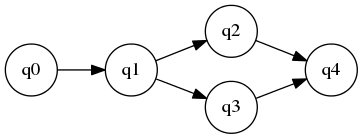
\includegraphics{tex/ejemplo_dibujo.png}
\end{center}
¿Cómo ordenar por relevancia los vértices?¿En qué orden aparecerán las páginas?


Para poder determinar qué páginas son más importantes vamos a suponer un paseo aleatorio por los vértices (los internautas navegan al azar siguiendo los enlaces) de forma que una mayor acumulación en ciertos vértices indicará que son más importantes.


\obs No funciona literalmente, hay que hacer modificaciones.

A la larga esto converge...
\begin{center}
	\centering
	\inputtikz{grafos_mod}
\end{center}




Como había 360 al principio parece que:


\begin{itemize}
	\item Probabilidad de estar en 1 es $\frac{144}{360} = \frac{2}{5}$
	\item Probabilidad de estar en 2 es $\frac{144}{360} = \frac{2}{5}$
	\item Probabilidad de estar en 3 es $\frac{72}{360} = \frac{1}{5}$
\end{itemize}
	Según esto 1 y 2 son igual de importantes y 3 es la mitad de importante.

	La distribución que pensamos que da el límite es estacionaria (no cambia con el tiempo).



% Empieza clase del 4 de Febrero

Recordamos que en la red anterior cuando el tiempo tiende a infinito parece que la distribución de personas se estabiliza.


Parece además que sea cual sea la distribución inicial llegamos a proporciones similares. En este caso llegamos a la distribución límite $\left(\frac{2}{5},\frac{2}{5},\frac{1}{5}\right)$, que es una distribución estacionaria (no varía con el tiempo).

\section{Propiedades de los paseos aleatorios}

\textbf{¿Esta simulación con paseos aleatorios siempre sirve para ordenar los vértices (páginas web)?}

Debemos estudiar las siguientes preguntas:

\begin{itemize}
	\item ¿Existe siempre una distribución estacionaria?
	\item Si existe una distribución estacionaria ¿es única?
	\item El procedimeinto, ¿Da lugar siempre a una distribución límite?
	\item Si la distribución límite existe, ¿Es independiente de la distribución inicial?

\end{itemize}

Vamos a analizarl estas preguntas y sus respuestas una a una.

\subsection{Si existe una distribución estacionaria ¿es única?}
\label{P2}

\begin{center}
	\centering
	\inputtikz{grafosIncomunicados}
\end{center}
% nodo 4 es internet oscura

Como desde un lado de la red no se puede acceder al otro podemos decir que estas dos distribuciones son estacionarias:

$(1, 2, 3, 4, 5, 6, 7)$

$(\frac{2}{5},\frac{2}{5},\frac{1}{5}, 0, 0 , 0, 0)$ es estacionaria.

$(0, 0, 0, 0, \frac{1}{5}, \frac{2}{5}, \frac{2}{5})$ es estacionaria.


\subsection{¿Existe siempre una distribución estacionaria?}

\begin{example}{Sencillo}

	\begin{center}
		\centering
		\inputtikz{grafo3nodosSimpleTik}
	\end{center}

	Si pones todos en un nodo oscila:

	$1\; 0\; 0 \rightarrow 0\; 0\; 1 \rightarrow 0\; 1\; 0 \rightarrow 1\; 0\; 0$

	Se puede argumentar que con una distribución inicial uniforme si funciona:

	$\frac{1}{3} \; \frac{1}{3} \; \frac{1}{3} \; \rightarrow \frac{1}{3} \; \frac{1}{3} \; \frac{1}{3} \; $

	Pero esto no es verdad para cualquier grafo: partiendo de la equidistribución no se tiene la convergencia en general.

	\begin{center}
		\centering
		\inputtikz{grafo4nodosTik}
	\end{center}


	$(\frac{1}{4},\frac{1}{4},\frac{1}{4},\frac{1}{4}) \rightarrow (\frac{1}{2},\frac{1}{4},\frac{1}{4}, 0) \rightarrow (\frac{1}{4},\frac{1}{4},\frac{1}{2},0)$ oscila como antes

	\textbf{La respuesta es negativa en general}

\end{example}


\subsection {Si la distribución límite existe, ¿Es independiente de la distribución inicial?}


Basta usar como distribución inicial las distribuciones estacionarias que vimos para la segunda pregunta \ref{P2}.

\begin{obs}

Para el grafo de \ref{P2} se puede probar que $\exists$ límite:

$$(1-t)\left(\frac{2}{5},\frac{2}{5},\frac{1}{5},0,0,0,0\right) + t \left(0,0,0,0,\frac{1}{5},\frac{2}{5},\frac{2}{5}\right) \;\;\; 0 \leq t \leq 1 $$

son infinitos contraejemplos como los necesarios para la segunda pregunta \ref{P2} y la cuarta.

\end{obs}


\textbf{Spoiler} P1 es verdad y "perturbando" un poco el grafo (de manera muy sencilla) todas las preguntas tienen respuesta afirmativa.



\section{Cadenas de Markov}

\begin{defn}[Cadena de markov]
	Es una sucesión de variables aleatorias $\{X_n\}_{n=0}^{\infty}$ que toman valores en un conjunto numerable S (\textbf{conjunto de estados}) tal que
	$$Prob(X_{n+1} = V | X_n = U) = Prob(X_{n+1} = V | X_n =U , X_{n-1} = U_{n-1} , ... , X_0 = U_0)$$
	para cualesquiera $n \geq 0$ $U,V,U_0,.... ,U_{n-1} \in S$
\end{defn}


\obs Además supondremos que esta probabilidad no depende de n.


\textbf{Idea intuitiva: } n es el tiempo discretizado, lo que ocurra mañana depende con cierta probabilidad de lo que ocurre hoy sin que importe conocer la historia anterior.

Decir que no depende de n es decir que según pasa el tiempo, las reglas no cambian.

\begin{example}
	$X_n =$ suma de puntuaciones el día $n$ al tirar un dado cada día.

	El conjunto de todos los estados serían todas las puntuaciones posibles . (S = naturales)

	Sabiendo lo que llevo acumulado hoy, tengo una cierta probabilidad de obtener mañana diferentes resultados, pero no depende de lo que ocurrió ayer; no me importa cómo he llegado a sumar lo que llevo hoy.
\end{example}

\begin{example}[2]
	S = puntuaciones en el tenis.\\
	$X_n =$ puntuación el en punto n\\
	Suponemos que el jugador A tiene prob $p > 1/2$ de ganar cada punto.\\
	Pensando un poco las puntuaciones en el tenis vemos que S solo puede tener 20 elementos.\\
	S= puntuaciones numéricas, deuce, advantages(A o B) , victoria (A o B).\\
	Se puede comprobar que:
	$$Prob(\text{victoria A}) = \frac{p^4 \cdot(1- 16(1-p)^4)}{p^4 - (1-p)^4}$$
	Esto es como curiosidad, ver que con tener sólo un poco más de probabilidad de ganar un punto, la probabilidad de ganar un juego y un set va creciendo.
\end{example}




Si $|S| = \infty$ entonces la cadena de Markov es infinita y se supone $S = \ent^+ (\nat -\{0\})$


Si $|S| < \infty$ entonces la cadena de Markov es finita y se supone $S =\{1,2,...,N\}$

\begin{defn}[Probabilidad de transición]
	del estado i al j
	$$P_{ij} = Prob(X_{n+1} = j| X_n = i) = Prob (X_1 = j| X_0 = i)$$
\end{defn}

Los $P_{ij}$ forman la \textbf{matriz de transición}.

\newpage
\textbf{Propiedades}
\begin{enumerate}
	\item $\sum_{j \in S} P_{ij} = 1$
	\item $Prob(X_1 = j)= \sum_{i \in S} Prob(X_0 = i)P_{ij}$\\
\end{enumerate}

\begin{proof}
	\begin{enumerate}
		\item $\sum_{j \in S} P_{ij} = \sum_{j\in S} Prob(X_1 = j | X_0 = i) = Prob (X_1 \in S | X_0 = i) = 1$
		\item Utilizando la ley de la probabilidad total

		$$Prob(X_1 = j) = \sum_{i \in S} Prob (X_0 = i) \cdot Prob(X_1 = j| X_0 = i)$$
	\end{enumerate}
\end{proof}

	\begin{defn}[Ley de la probabilidad total]
		Sea  $\{A_1, A_2,...,A_n\}$ una partición de $\Omega$ con $P(A_i)>0 \ \forall i=1,2,...,n$. Entonces, $\forall B \subset \Omega$ medible (perteneciente a $\algb{M}$):
		\[
		P(B)=\sum_{i=1}^{n}P(B\cap A_i)=\sum_{i=1}^{n}P(B|A_i)P(A_i)
		\]
		Esta propiedad se obtiene de despejar de la formula de la probabilidad condicionada:
		\[P(A|B)=\frac{P(A \cap B)}{P(B)}\]
	\end{defn}


De las dos propiedades deducimos que:
\begin{itemize}
	\item \textbf{(prop.1)} La matriz de transición $P_{ij} i,j \in S$ tiene elementos $0 \leq P_{ij} \leq 1$ y la suma de los elementos de cada fila es 1.
	\item Escribiendo ($\Pi_0$) = ${Prob (X_0 =i)}_{i \in S}$ como vector fila, y ($\Pi_n$) = ${Prob (X_n =i)}_{i \in S}$

	Entonces por \textbf{(prop.2)} : ($\Pi_1$) $ = (\Pi_0)\cdot P$ (P = matriz de transición)
\end{itemize}

De la misma forma $(\Pi_2) = (\Pi_1) \cdot P$, etc...

Iterando nos queda:
$$\left(\Pi_n\right) = \left(\Pi_0\right) \cdot P^n$$

Ahora vemos cómo aplicar esto a las páginas web.


Teniendo en cuenta que en la realidad la P sería una matriz de $3\cdot 10^{13} \times 3\cdot 10^{13}$ la forma más fácil de calcular $P^n$ es con la forma canónica de Jordan. Veámoslo con un ejemplo.
\begin{example}[1]{}

%Hola kasner, tienes dos opciones, la que creo que quieres es la que no está comentada, q es la que está justo despues de la comentada. Ala, me debes un café.

%\begin{figure}[ht]
%	\centering
%	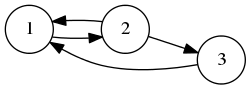
\includegraphics{tex/grafo3nodos.png}
%	\caption{Figurita molona}
%\end{figure}

	\begin{center}
	\centering
	\inputtikz{grafo3nodosTik}
\end{center}


	S= páginas web (vértices)\\
	$P_{ij}$ = probabilidad de , estando en la página i, llegar a la página j en el instante siguiente.

	$$Prob(X_1 = (2)| X_0 = (1)) = 1$$
	$$P =\left(\begin{matrix}
	0 & 1 & 0\\
	1/2 & 0 & 1/2\\
	1 & 0 & 0
	\end{matrix}\right)$$

	Hacemos Jordan:
	$$P = C^{-1} \left(\begin{matrix}
	1&&\\
	&z&\\
	&&\overline{z}
	\end{matrix}\right) C$$
	Haciendo los cálculos nos queda $z = \frac{1}{\sqrt{2}}\cdot e^{\frac{3\pi i}{4}}$

	Por lo tanto:
	$$P^n =  C^{-1} \left(\begin{matrix}
	1&&\\
	&z^n&\\
	&&\overline{z}^n
	\end{matrix}\right) C \stackrel{n\rightarrow \infty}{\rightarrow}  C^{-1} \left(\begin{matrix}
	1&&\\
	&0&\\
	&&0
	\end{matrix}\right) C = \left(\begin{matrix}
	2/5&2/5&1/5\\
	2/5&2/5&1/5\\
	2/5&2/5&1/5
	\end{matrix}\right) = L$$
	Esto implica que:
	$$\lim_{n\rightarrow\infty}\left(\Pi_n\right) = \lim_{n\rightarrow\infty}\left(\Pi_0\right)\cdot P^n = \left(\Pi_0\right)\cdot L =( \begin{matrix}
	2/5&2/5&2/5
	\end{matrix})$$
	Que es independiente de $\Pi_0$
\end{example}

\begin{example}[2]

	\begin{center}
		\centering
		\inputtikz{grafo4nodosTik}
	\end{center}

	$$P = \left( \begin{matrix}
	0 & 1 & 0 & 0\\
	0 & 0 & 1 & 0\\
	1 & 0 & 0 & 0\\
	1 & 0 & 0 & 0\\
	\end{matrix}\right)= C^{-1} \left(\begin{matrix}
	1&&&&\\
	&w&&&\\
	&&\overline{w}&\\
	&&&0
	\end{matrix}
	\right)\cdot C$$
	$w = e^{\frac{2\pi i}{3}}$ , si seguimos calculando las potencias de $w$ y de $\overline{w}$ vemos que van oscilando entre los valores $w , \overline{w} , 1$, por lo que vemos que en este caso $P^n$ no tiene límite.
	$$\exists\left(\Pi_0\right) : \nexists \lim \left(\Pi_0\right)\cdot P^n$$
	Sin embargo con $(\Pi_0) = (\begin{matrix}
	1/3&1/3&1/3&0
	\end{matrix}) $ se comprueba $(\Pi_0) = (\Pi_0)\cdot P$


	Con lo que para ese $(\Pi_0)$ si tenemos límite.Ya veremos más adelante cómo se llaman este tipo de distribuciones.
\end{example}

Lo que hemos comprobado con estos dos ejemplos es que si conocemos la forma canónica de Jordan podemos saber si tenemos convergencia o no.

\paragraph{Resumen de lo visto hasta ahora}
\begin{itemize}
	\item Cadenas de Markov $\begin{cases}
	(\Pi_0) = \{P(X_0 = i)\}_{i \in S} \rightarrow \text{\textbf{distribución inicial}}\\
	P = \text{Matriz de transición}
	\end{cases}$
	\item Distribución de probabilidad en el instante $n = (\Pi_0)P^n$
	\item $P^n$ se calcula con la forma canónica de Jordan
	\item En general queremos que exista la \textbf{distribución límite} : $\lim_{n\rightarrow\infty} (\Pi_0) P^n$
\end{itemize}

\obs Si existe $\left(\Pi\right) = \lim \left(\Pi_0\right) P^n$ entonces $\left(\Pi\right) = \left(\Pi\right) P$
\begin{proof}
	$\left(\Pi\right) = \lim\left(\Pi_0\right) P^{n+1} = \left(\lim \left(\Pi_0\right)P^n\right)P = \left(\Pi\right) P$
\end{proof}

\begin{defn}[Distribuciones estacionarias]
	Se dice que $\left(\Pi\right)$ es una distribución de probabilidad estacionaria si:
	$$\left(\Pi\right)\cdot P = \left(\Pi\right)$$
\end{defn}

\obs Con estas distribuciones podemos calcular el límite y estudiar la convergencia sin utilizar la forma canónica de Jordan.


Recordando las preguntas que nos hicimos con las propiedades de los paseos aleatorios vemos que, experimentalmente, las cadenas de Markov muy interconectadas responden afirmativamente a esas preguntas.

Vamos a ver dos versiones de lo que se entiende por \textbf{conexión} de una cadena de Markov
\newpage
\begin{itemize}
	\item \begin{defn}[Irreducible]
		Se dice que una cadena de Markov es \textbf{irreducible} si se puede ir de un estado a otro en un número finito de pasos. Es decir
		$$\forall i,j \in S\text{    }\exists k : P(X_k = j| X_0 = i) \neq 0$$
		Otra forma de definirlo es con la matriz de transición:
		$$\forall i,j \in S \text{    }\exists k: (P^k)_{ij} \neq 0$$
	\end{defn}
	\item \begin{defn}[Regular]
		Se dice que una cadena de Markov es \textbf{regular} si existe un número de pasos tal que dándolos se puede pasar de un estado a cualquier otro. Es decir:
		$$ \exists k : P(X_k = j| X_0 = i) \neq 0  \forall i,j \in S $$
		Otra forma de definirlo es con la matriz de transición:
		$$\exists k : \text{ todos los elementos de} P^k \text{ son positivos.}$$
	\end{defn}
\end{itemize}


Los experimientos muestran que en casos con mucha "interconexión" $\exists \lim (\Pi_0)P^n$ y no depende de $(\Pi_0)$.

En principio sabemos resolver cada problema, en caso finito, con la forma canónica pero esto no es muy práctico.
\subsection{Teoremas}
\begin{theorem}[Teorema 1]
	\label{Markov_tma1}
	Una cadena de Markov finita siempre tiene al menos una distribución estacionaria.
\end{theorem}

	\obs Teorema1 $\iff$ 1 es autovalor de P con autovector por la izquierda.


	Para demostrarlo vamos a utilizar el \textbf{Tma. del punto fijo de Browner}.


	Recordemos este teorema:
	$$f: B^n \rightarrow B^n  \text{  B bola cerrada en }\real^n \implies \exists \overrightarrow x \in \real^n : f(\overrightarrow x ) = \overrightarrow x$$
	No vamos a demostrarlo formalmente. podemos verlo en el siguiente dibujo para dimensión 1.

	DIBUJO

	Vemos que $g(x) = f(x) - x$ por lo que para $g(x) = 0$ tenemos $f(x) = x$

	En dimensión dos no es intuitivo y en las demás dimensiones ya es muy difíci, por lo que vamos a creernoslo y punto.

	Una vez recordado esto ya nos podemos poner con la demostración del Teorema 1:
	\begin{proof}
	$$K = \{(x_1 , x_2, \ldots x_N) \in \real^n : \sum x_i = 1 , x_1 \geq 0\}$$

	Vemos que K es homeomorfo a la bola $B^{N-1}$

	Ejemplo N=2:
	(dibujo)
	Es obvio que es homeomorfo porque es un segmento.

	Ejemplo N=3:
	(dibujo)
	K sería el triángulo. Con una proyección tendría el triángulo en el plano xy.
	Una vez pasado a $\real^2$ , para demostrar que es homeomorfo a $B^2$ solo habría que "estirarlo" hasta la bola.

	Entonces tenemos K homeomorfo a $B^{N-1}$. Multiplicamos los elementos de K por P.

	$x \in K \implies (x)\cdot P \in K$ porque como la suma de los elementos de las filas de P=1 $\implies (x)\cdot P$ sigue perteneciendo a K.

	Y teniendo esto es fácil terminar la demostración ya que por el teorema de Brouwer $enxists (x) : (x) = (x)\cdot P$
\end{proof}

\begin{theorem}[Teorema 2]
	\label{Markov_tma2}
	Para una cadena de Markov finita regular $\exists \lim (\Pi_0) P^n$ y el resultado no depende de $(\Pi_0)$ y es la única distribución estacionaria.
\end{theorem}

Para esta demostración vamos a utilizar el siguiete lema:
\begin{lemma}
	Tenemos la aplicación lineal
	$$F: \real^m \rightarrow \real^m$$
	y $\Omega = $ compacto que contiene a $\overrightarrow o$.

	Supongamos que $F(\Omega) \subset Int(\Omega)$. Entonces
	$$\forall \overrightarrow{x_0} \in \Omega , \overrightarrow{x_n} = F(\overrightarrow{x_{n-1}}) \text{ se cumple que } \overrightarrow{x_n} \rightarrow \overrightarrow o$$
\end{lemma}

La idea de porqué se cumple este lema es la siguiente:
Dibujo

Al ser F aplicación lineal , el $\overrightarrow o$ va al $\overrightarrow o$.

Si vas iterando muchas veces, al final F se va haciendo tan pequeña que tiende a $\overrightarrow o$

Creyéndonos el lema pasamos a la demostración del teorema 2.

\begin{proof}
	Tomamos K como en el Teorema 1.
		$$K = \{(x_1 , x_2, \ldots x_N) \in \real^n : \sum x_i = 1 , x_1 \geq 0\}$$
	y $f(x) = (x)\cdot P$

	Por el Teorema 1 $\implies \exists (\Pi)$ estacionaria $f(\Pi) = (\Pi)$. Pero todavía no sé si es única.

	\obs K no contiene al origen $\implies$ el lema no se aplica directamente pero hacemos una pequeña variación:

	$$\Omega = \{(x) - (\Pi) : (x) \in K\} \rightarrow \text{ compacto y convexo}$$

	Convexo: si tengo dos puntos, también tengo los puntos entre medias.


	Entonces
	$$\Omega \subset \{(x_1 , \ldots , x_N) \in \real^N : \sum x_i = 0\} = H$$

	Podemos identificar $H$ con $\real^{N-1}$ .

	Para explicar esto ponemos el ejemplo de una recta, que mirada desde cierta perspectiva, se ve como un punto, o un plano como una recta.

	Se cumple que $f(\Omega) \subset \Omega$ porque $f(K) \subset K$ y $\f(\Pi) = (\Pi)$

	Ahora vamos a demostrar que va al interior.

	$$Int(\Omega) = \{(x) - (\Pi) : (x) \in K, x_i >0\} [ = \text{ conjunto compacto - frontera}]$$
Por ser regular $\exists k : P^k$ tiene elementos positivos ($>0$). Entonces
$$f^k(\Omega) = f \circ f\circ . . . \circ f(\Omega) \subset Int(\Omega)$$

Ya que en otro caso habría puntos de la frontera y estos tienen alguna coordenada no nula.

Aplicando el lema a $f^k$ y tomando $(\Pi)$ estacionaria y $(x) = (\Pi_0)$ se tiene que
$$\lim_{n \rightarrow \infty} ((x) - (\Pi)) \cdot P^{kn} = (0)$$
Entonces
$$\lim_{n \rightarrow \infty} (\Pi_0) \cdot P^{kn} = (\Pi)$$
y finalmente
$$\lim_{n \rightarrow \infty} (\Pi_{kn}) = (\Pi)$$

Y el límite es único.

Por lo tanto, aplicando $P$ k-1 veces:
$$\lim_{n \rightarrow \infty} (\Pi_{n}) = (\Pi)$$
\end{proof}

\begin{example}
	$$\lim(\Pi_{2n}) = (\Pi) \implies \lim (\Pi_{2n})\cdot P = (\Pi)\cdot P \implies \lim(\Pi_{2n +1}) = (\Pi)$$
\end{example}


\begin{theorem}[Teorema 3]
	\label{Markov_tma3}
	Para cualquier cadena de Markov finita, el límite:
	\[\lim \frac{(\Pi_0)+(\Pi_1)+…+(\Pi_n)}{n+1}  \text{ (con }(\Pi_n) = (\Pi_0)P^n\text{)}\]
	existe y converge a una distribución estacionaria.

\end{theorem}

\begin{proof}

	$$ S_n = \frac{1}{n+1} \sum\limits^{n}_{k=0} P^k \;\;\;\;\; S_n \text{ es una matriz} $$

	La suma de los elementos de cada fila de $P^k = 1$. Como hacemos promedio $\Rightarrow$ A $S_n$ le pasa lo mismo y sus elementos están en $[0,1]$.

	$$B-W \Rightarrow \exists n_j : S_{n_j} \text{ converge } (\exists \lim_{j \rightarrow \infty} S_{n_j})$$

	Usando el teorema de Boltzano Weirestrass, si no existiera el límite de $S_n$ existirían $n_j, m_j$ con $\lim S_{n_j} \neq \lim S_{m_j}$.

	$$L_1 = \lim S_{n_j} \;\;\;\;\;\; L_2 = \lim S_{m_j}$$

	$$L_1 P = L_1 \;\;\;\;\;\; P L_2 = L_2$$
	$$L_1 S_{m_j} = L_1 \;\;\;\;\;\; S_{n_j} L_2 = L_2$$

	$$ \convs[][j][\infty] $$

	$$L_1 L_2 = L_1 \;\;\;\;\;\; L_1L_2 = L_2 \Rightarrow L_1 = L_2 $$

\end{proof}

\begin{example}

\begin{center}
	\inputtikz{markov/triangulos_separados}
\end{center}

Tenía muchas distribuciones estacionarias: $\exists \lim(\Pi_0)P^n$ pero depende de $(\Pi_0)$.

No es irreducible $\Rightarrow^{\text{(lo veremos)}}$ se pierde la unicidad de la distribución estacionaria.

\end{example}

\begin{example}

\begin{center}
	\inputtikz{markov/triangulo_con_entrada}
\end{center}

No es regular, por ello hay dependencia en $(\Pi_0)$, no es regular, no existe $\lim(\Pi_0) P^n$ en general. Pero $\exists \lim$ del tercer teorema \ref{Markov_tma3} y en $\left(\frac{1}{2},\frac{1}{3},\frac{1}{3},0\right)$.

\end{example}


\subsection{Page Rank Algorithm}

\begin{center}
	\inputtikz{markov/red_pagerank}
\end{center}


$$\text{Modelo: } P_y = \left\{
	\begin{array}{ll}
		0  & \mbox{si} \text{no hay enlace de i a j} \\
		\frac{1}{\text{nº de enlaces salientes}} & \mbox{si} \text{hay enlace de i a j}
	\end{array}
\right.
$$

P es una matriz $N \times N$ $N = 3 \, 10^{13}$.

\textbf{Idea} Si estuviéramos en las hipótesis del Teorema 2 \ref{Markov_tma2} entonces  $(\Pi_0) P^{\text{nº grande}}$ aproximaría la distribución de probabilidades de estar en cada página (navegando por los enlaces al azar) (en la práctica $50 \leq \text{nº grande} \leq 100$).


Esencialmente lo que se hace para estar las hipótesis del Teorema 2 \ref{Markov_tma2} es cambiar ceros por números pequeños. Así se convierte en una matriz con elementos > 0, con lo que se cumple la definición de regular con $k=1$.

Concretamente se cambia la $P$ original por:

$$P_{\epsilon} = (1-\epsilon) P + \epsilon E \;\;\;\; \text{ siendo }E = \text{matriz con todos sus elementos } \frac{1}{n}$$

\begin{example}

\begin{center}
	\inputtikz{markov/grafo_2-ciclo}
\end{center}

	$$P = \left( \begin{array}{ccc}
0 & 1 & 0 \\
0 & 0 & 1 \\
0 & 1 & 0 \end{array} \right)$$

No podemos sustituir directamente los 0 por ε ya que entonces no sumarían 1 las filas.

Por tanto debemos sustituir los 0 por δ y ajustamos los elementos no nulos para que sumen 1.

$$P_{\delta} = \left( \begin{array}{ccc}
\delta & \;\; 1-2\delta \;\; & \delta \\
\delta & \;\; \delta \;\;& 1 - 2 \delta\\
\delta & \;\; 1 - 2 \delta \;\; & \delta \end{array} \right)$$



$\delta = \frac{\epsilon}{3}$ (solo notación) $\Rightarrow$ esta última matriz es:


$$P_{\delta}= (1-\epsilon)\left( \begin{array}{ccc}
0 & 1 & 0 \\
0 & 0 & 1 \\
0 & 1 & 0 \end{array} \right) + \epsilon \left( \begin{array}{ccc}
1/3 & 1/3 & 1/3 \\
1/3 & 1/3 & 1/3 \\
1/3 & 1/3 & 1/3 \end{array} \right)$$


Es facil comprobar (ej) que $P_{\epsilon}$ tiene filas con suma 1. Además, si $\epsilon$ pequeño, $P_{\epsilon} ≈ P$.

Lo que hacen los $\epsilon$ es representar la posibilidad de que alguien salte a una página aleatoria.

\begin{center}
	\inputtikz{markov/grafo_2-ciclo_completo}
\end{center}


En este mismo ejemplo vamos a ver qué pasa con la convergencia:

Intuitivamente los nodos 2 y 3 deberían tener probabilidad $\frac{1}{2}$ y el nodo 1, probabilidad 0.

Si partimos de $\left(\Pi_0\right)= \left(x,y,z\right)$ , sin hacer ningún cambio en $P \implies$
$$\left(\Pi_1\right) = \left(\Pi_0\right)P = \left(0,x+z,y\right)\rightarrow \left(\Pi_2\right) = \left(0,y,x+z\right) \rightarrow ..... \rightarrow \text{oscila}$$

¿Qué pasa si lo miramos con $P_{\epsilon}$?

$$\lim\limits_{\epsilon \rightarrow 0} \left(\Pi_0\right)P_{\epsilon} = \lim\limits_{\epsilon \rightarrow 0}\left(\frac{\epsilon}{3}, \frac{1- 2\epsilon/3}{2-\epsilon}, \frac{1-\epsilon +  \epsilon^2/3}{2- \epsilon}\right)$$

Para $\epsilon \rightarrow 0$ tendremos algo cercano a la intuición $\left(0, \frac{1}{2}, \frac{1}{2}\right)$
\end{example}


Hasta aquí la parte teórica pero \textbf{¿realmente se puede hacer algo similar con $N = 3\cdot 10^{13}$?}

En vez de $\lim\left(\Pi_0\right)P_{\epsilon}^n$ , se calcula $\left(\Pi_0\right)P_{\epsilon}^{n.grande} $ con $\left(50 \leq \text{ n grande }\leq 100\right)$

Y ahora vamos a ver el coste que tiene la operación $\left(\Pi_0\right)P_{\epsilon} = \left(1-\epsilon\right)\left(\Pi_0\right)P + \epsilon\left(\Pi_0\right)E$ :

Vemos que $\epsilon\left(\Pi_0\right)E$ no requiere ninguna operación. Si lo vemos en el ejemplo de N = 3:

$$(x , y , z)\cdot \left( \begin{array}{ccc}
1/3 & 1/3 & 1/3 \\
1/3 & 1/3 & 1/3 \\
1/3 & 1/3 & 1/3 \end{array} \right) = (1/3 , 1/3 , 1/3)$$

\obs $\frac{x}{3} + \frac{y}{3} + \frac{z}{3} = \frac{1}{3}(x + y + z)$ y $(x +y +z)=1$ porque son las probabilidades de pasar a $x$ , a $y$ o a $z$.

En general , $\epsilon(\Pi_0)E = (1/N , 1/N, ....,1/N)$

¿y la parte de $(1-\epsilon)(\Pi_0)P$?

Es sencilla porque $P$ está llena de ceros.
\begin{itemize}
	\item Si cada página tiene k enlaces, P tiene sólo $k\cdot N$ elementos no nulos
	\item Cada iteración $(\Pi_n) =(\Pi_{n-1})$ lleva del orden de $k\cdot N$ operaciones, y esto es factible incluso en nuestro ordenador.
\end{itemize}


\textbf{¿Cuánto de pequeño debería ser $\epsilon$?}

Matemáticamente debería tomarse $\epsilon\rightarrow 0$ pero en la práctica, cogiendo un $\epsilon$ muy pequeño la convergencia es muy lenta.

Google dice que usa $\epsilon = 0.15$.

\textbf{Curiosidad} : Una prueba de que Google no sólo utiliza este algoritmo para dar prioridad a sus páginas es lo siguiente:

Algunas empresas hacen \textit{link farming} (interconectarse aún sin tener nada que ver) ya que de esta forma, según el algoritmo, deberían subir de prioridad.

\begin{center}

	\inputtikz{markov/link_farming}

\end{center}

Pero google puede detectarlo y eliminarlo, por lo que queda claro que utiliza otras herramientas.

\textbf{Propuesta de ejercicios:}

\textbf{1)}


	Simular con un programa(en el lenguaje que queramos, mejor C o C++) una red grande (p.ej $N= 10^6$) "aleatoria" , de modo que cada página tenga 10 enlaces , y ver cuánto se tarda en hallar $(\Pi_0) P_{\epsilon}^{100}$
	Chamizo tardó 70 segundos.



\textbf{2)}


	Crear un generador de textos aleatorios en un idioma.

	Lenguaje de programación recomendado: Phyton

	¿Cómo hacerlo?
	\begin{enumerate}
		\item coger un texto largo en el idioma que queramos
		\item Estados = pares de de palabras consecutivas
		\item Unir estados de forma aleatoria.
	\end{enumerate}
	P.ejemplo: [a manos] $\rightarrow$ [manos llenas] $\rightarrow$ [llenas de] / [llenas con] ....

\subsection{Cabos sueltos}
 Repasando los teoremas \ref{Markov_tma2} \ref{Markov_tma3} vemos que han dejado algunos cabos sueltos.
\begin{itemize}
	\item ¿Qué se necesita para la unicidad de la distribución estacionaria?
	\item ¿qué ocurre con las cadenas de Markov infinitas?
\end{itemize}

Hay un teorema que responde a estas dos cosas.
La idea es:
	En una cadena de Markov finita irreducible $\implies$ existe una única distribución estacionaria.

	Pero esto no se cumple en las infinitas.
	\begin{example}[cadena infinita en el que no existe distr.estacionaria]
		Consideramos los números naturales:
		\begin{center}

			\inputtikz{markov/grafoInfIrre}

		\end{center}
		$$S = \ent ^+$$
		Vemos que efectivamente es irreducible.

		Vamos a comprobar que no existe una distribución estacionaria:

		Suponemos que tengo una distribución estacionaria para llegar a una contradicción:

		$$(\Pi) = (x_1, x_2, x_3...)$$
		$$\sum x_i = 1$$

		Vemos que
		$$
		\begin{cases}
		x_1 = \frac{1}{2} x_2 \implies x_2 = 2x_1\\
		x_2 = x_1 + \frac{1}{2} x_3 \implies x_3 = 2x_1\\
		x_3 = \frac{1}{2} x_2 + \frac{1}{2} x_4 \implies x_4 = 2x_1\\
		.\\
		.\\
		.\\
		\end{cases}$$
		Esto lleva a una contradicció porque el resultad esperado si existiera la distribución estacionaria sería:
		$$x_1 + \sum_{n=2}^{\infty} 2 x_1 =1$$
		Pero esto es imposible.
	\end{example}



	De esto de deduce que lo importante para la existencia y unicidad de distribuciones estacionarias no es tanto que se pueda ir de un estado a otro si no que el \textbf{tiempo medio de retorno} sea finito.

	\begin{defn}[Tiempo medio de retorno]
		Es el tiempo de retorno al estado i y se define como:
		$$m_i = E[T_i|X_0 = i]$$

		Siendo $T_i = inf{n>0 : x_n = i}$ el tiempo mínimo en volver.
	\end{defn}

	\obs Para cadenas de Markov finitas irreducibles $m_i < \infty$

	\begin{theorem}[Teorema 4]
		\label{Markov_tma4}
		Para una cadena de Markov irreducible (finita o infinita)
		$$\exists \text{ distribución estacionaria } \iff m_i <\infty \text{ para algún i}$$
		Además $m_i<\infty$ implica que la distribución estacionaria es:
		$$(\Pi) = (\frac{1}{m_1}, \frac{1}{m_2},\frac{1}{m_3}, .....)$$
		y es única.
	\end{theorem}
	\obs Si $m_i$ existe para algún estado, existe para todos.

	\begin{example}
		Recordemos el ejemplo de :
			\begin{center}
				\centering
				\inputtikz{grafo3nodosTik}
			\end{center}

		Tenemos que $(\Pi) = (\frac{2}{5}, \frac{2}{5}, \frac{1}{5})$. El teorema nos permite ver que:
		\begin{itemize}
			\item $\frac{1}{2/5} = \frac{5}{2}$ es el tiempo medio (n. de clicks) para volver al estado 1 partiendo del estado 1.
			\item Lo mismo para 2
			\item $\frac{1}{1/5 = 5}$ es el tiempo medio de retorno para el nodo 3.
		\end{itemize}
	\end{example}

	Ahora vamos a ver que aplicando la \textbf{Ley Fuerte de los Grandes Números} a este tema, se cumple casi seguro que:
	$$\lim_{n \rightarrow \infty} \frac{N_n (i)}{n} = \frac{1}{m_i}$$

	Siendo $N_n (i)$ el número de veces que hemos vuelto a i en n Unidades de Tiempo.

	\obs No se cumple al $100\%$ ya que son variables aleatorias.

	\begin{example}
		Con el mismo grafo del ejemplo anterior, si desde 1 hago n licks , con n grande, típicamente ha vuelto a 1 del orden de $\frac{n}{5/2} = \frac{n}{m_1}$
	\end{example}

	\textbf{Conclusión :} $N_n (i) \sim \frac{n}{m_i}$




\section{Una cadena de Markov infinita: Movimiento bronniano}

\begin{center}
	\inputtikz{markov/movimiento_bronniano}
\end{center}

Modela, entre otros, el movimiento de párticolas pequeñas (polen) sobre un líquido, que siguen un "camino aleatorio" al ser golpeadas por muchas moléculas.

Nuestro ejemplo concreto: Modelo de partículas que se mueven al azar a derecha o izquierda (paseo aleatorio).

Los estados son $S = \mathbb{Z}$. Y la matríz de transición cumple:


$$ P_{i,i-1} = P_{i, i+1} = \frac{1}{2} \;\;\;\;\; P_{i,j} = 0  \text{  (En el resto de casos)} $$


Para estudiar el movimiento bronniano nos gustaría que los estados estuvieran "muy pegados" formando un contínuo $\mathbb{R}$. También nos gustaría hacer continuo el tiempo.


Calculemos el nº de visitas (retornos) esperados al origen = 0.

Probabilidad de volver en tiempo $ = 2 \equiv P(X_{2} = 0 | X_{0} = 0) = \frac{1}{2^2} 2 $

Probabilidad de volver en tiempo $ = 4 \equiv P(X_{4} = 0 | X_{0} = 0) = \frac{1}{2^4} \binom{4}{2} $

Probabilidad de volver en tiempo $ = 2j \equiv P(X_{2j} = 0 | X_{0} = 0) = \frac{1}{2^{2j}} \binom{2j}{j} $


Entonces $ N_{n} (0) = \sum\limits_{2j \leq n} \frac{1}{2^{2j}} \binom{2j}{j} $

$$ \lim_{n \rightarrow \infty} \frac{N_{n}(0)}{n} = 0 $$

Este cálculo requiere usar aproximaciones finas de factorial (Stirling).

Podemos ver entonces que no existe una distribución estacionaria ya que $\frac{1}{m_i} = 0 \Rightarrow m_i = \infty$.



Teniendo $P(X_{n} = j)$ con la matriz de transición se puede calcular facilmente $P(X_{n+1} = j)$.

$$ P(X_{n+1} = j) = \frac{1}{2} P(X_{n} = j-1) + \frac{1}{2} P(X_{n} = j+1) $$


Queremos que los tiempos en vez de ser 0,1,2,3,... dean $0h, 1h, 2h, ...$ con $h$ pequeño y que los estados sean $\epsilon \mathbb{Z} = \{ 0\epsilon, \pm 1\epsilon, \pm 2\epsilon, ... \}$ con $\epsilon$ pequeño. Además queremos que en tiempo acotado $hn (=1)$ nos hayamos movido típicamente un espacio $\epsilon j$ acotado.

En el paseo aleatorio en $\mathbb{Z}$ se prueba que típicamente en n pasos se llega a distancia $c \sqrt{n}$. tiempo $≈ \sqrt{\text{dist}}$, lo que sugiere que $h ≈ \epsilon^2$.


Elijamos $h = \frac{1}{2} \epsilon^{2}$ (si en vez de $\frac{1}{2}$ escogieramos otra constante apenas habría cambios):


$$ \frac{P(X_{n+1} = j) - P(X_{n} = j)}{h} = \frac{P(X_{n} = j-1) + P(X_{n} = j+1) - 2 P(X_{n} = j)}{\epsilon^2} $$

Queremos que cuando $h \rightarrow 0$ $P(X_{n} = j) = u(x, t) j \in \mathbb{Z} \;\; n \in \mathbb{Z}^{+} \cup \{0\} $ ($ x = j\epsilon, t = nh $).


Teniendo en cuenta que $h \rightarrow 0 $y $\epsilon \rightarrow 0$.

$$ \frac{u(x, t h) - u(x,t)}{h} = \frac{u(x-\epsilon, t) + u(x + \epsilon, t) - 2 u (x, t)}{\epsilon^2} $$


$$ u_{t} = u_{xx} $$

\begin{op}{Ecuación del calor en R}
\begin{cases}
	u_{t} = u_{xx} \;\;\;\; x \in \mathbb{R} t > 0 \\
	u(x,0) = f(x) \;\;\; \leftarrow \text{distribución inicial}
\end{cases}
\end{op}


Como las probabilidades de la cadena de Markov siempre suman (integran) 1 esto debe ser verdad para cualquier tiempo.

Es decir:

$$ \int_{\mathbb{R}} f(x)dx = 1 \Rightarrow \int_{\mathbb{R}} u (x,t) dx = 1 \text{ para cualquier t}$$

Si u resuleve la ecuación del calor :

$$ \text{SOL:} u(x,t) = \frac{1}{\sqrt{4\pi t}} \int_{-\infty}^{infty} f(y) e ^{-(x-y)^2 / ut} dy $$

Si $e \neq \frac{1}{2}$, si uno pone otro número, aparece una constante en $u_{t} = e_{2} u_{xx}$.







